\section{Results}
\subsection{Tracking performance}
The presented model splits the tracking problem into growth cone detection and
identity association. A representative example of detections is shown in Figure
\ref{R_modelresults} B. Given the temporal stack of five image tiles, the
detection model accurately identifies growth cones in PDMS micro structure
timelapse frames. False positive detections made by the model are often
ambiguous image regions that may be interpreted as positives under less
conservative ground truth labelling. On the test set, the detector reaches a
precision of 0.73, and recall of 0.79. F1 score at a confidence threshold of
0.79 is 0.76 (Figure \ref{R_modelresults} C). A both deeper and wider CNN
architecture did show decreased performance. The ensuing step of identity
association was performed in a graph framework optimizing for minimum cost flow
solutions. Matching detection performance in tracking is challenging as in
addition to detection, identity switches, object occlusions, and suitable
identity creation-, and termination need to be considered. Using the multiple
object tracking benchmarks proposed in \cite{mot_benchmark_2015}, our tracker
achieves identity precision, recall and F1 score of 0.73, 0.68, 0.71,
respectively, which is a reasonably small drop from detection performance
(Figure \ref{R_modelresults} D). The commonly used MOTA (multiple object
tracking accuracy) metric which considers the number of false positives, false
negatives (including identity), and identity switches normalized to the number
of ground truth labels was 0.61. A more intuitive measure of tracking
performance is visualized by the top bar in Figure \ref{R_modelresults} D,
indicating the proportion of growth cones mostly tracked (0.57), partially
tracked (0.23), and mostly lost (0.2). 

Although not utilized for our application of the tracking model, axons can be
reconstructed from the growth cone track, assuming that outgrowth followed the
shortest path between detections. A visualization of the reconstructions is
shown in Suppl. Figure \ref{SF_methods_expl} B.

\begin{figure}[h!]
    \includegraphics{R_modelresults.pdf}
    \caption[Growth cone tracking model performance]
        {Growth cone tracking model performance. \textbf{A} Loss and performance
        over 1500 training epochs. Dotted line refers to train set, solid line
        to test. The plotted loss was smoothed with an exponentially decaying
        kernel over 25 epochs, precision, recall, and F1 over 60 epochs.
        \textbf{B} Representative growth cone detection example. Dashed boxes
        are predicted, colored ones are ground truth. Scale bar = 90 $\rm \upmu
        m$. \textbf{C} Detection performance. The maximum F1 score for varying
        confidence thresholds on test set is indicated by the dot. The brown
        line shows performance for a model with wider and deeper architecture.
        Legend in A applies. \textbf{D} Model growth cone tracking performance.
        Identity precision and recall incorporate classification of correct
        identity. Each black dot represents the performance using one set of
        hyperparameters, the green dot represents the highest scoring set (see
        Table \ref{MCF_params}) where identity F1 was 0.71, MOT accuracy 0.61.
        MOT accuracy measures the number of false positives, false negatives,
        and identity switches normalized to the number of ground truth labels.
        The top bar visualizes the proportion of growth cones that were mostly
        tracked (green, $>$80\% identity lifetime tracked), mostly lost (brown,
        $<$20\%), and partially tracked (dark green, between 20-80\%).
        } 
    \label{R_modelresults}
\end{figure}

\subsection{Micro structure designs}
The tracking model described above was used for evaluating a set of 21 PDMS
micro structures designed for directing axon growth from multiple source regions
towards a common target. These designs are the result of unpublished previous
work extensively described in Supplementary Information 1. In short, the 21
designs test a set of presumably relevant variables that yield directional
axonal growth, including different types of 2-joints, joint placements and joint
frequencies. Figure \ref{R_designs} illustrates the specific features
implemented in the different designs. Design 05 on the right exemplifies the
general PDMS architecture composed of four source wells, the final lane,
the higher output channel with added diffusion wells and finally a target
stomach \parencite{forro}. 

\begin{figure}[h!]
    \includegraphics{R_designs.pdf}
    \caption[PDMS micro structure designs]
        {PDMS micro structure designs. The left illustration provides an
        overview of the 20 modelled micro structures including their
        distinguishing design features. Starting from Design 00 (D00), the arrows
        can be interpreted as an implemented design change. For example, D05 and
        D06 differ specifically in the number of 2-joints. For more details on
        the single designs see Suppl. Information 1. On the right, the D05 design is
        shown as an example. Filled white regions are openings, white lines
        indicate 6 $\upmu$m high channels, the black region represents the 75
        $\upmu$m high output channel (note discontinuity for illustrative
        reason). RGC spheroids are seeded in the source wells (S), the thalamic
        attractor is placed in the target well (T). Grid dimension 100 $\upmu$m.
        The magnification highlights the two main merging structures, 2-joints
        and final lane joints.} 
    \label{R_designs}
\end{figure}


\subsection{Between dataset variance}
The translocation of RGC growth cones was tracked over a period of five days to
infer the degree of directional growth through new PDMS micro structure designs.
The directionality was evaluated based on the A* distance-to-output channel over
time (see Methods \ref{inferring_directionality}). Figure \ref{R_more_metrics} A
shows this inference of directionality from output channel distances for
tracking axons in Design 05. Axons that grow towards the output channel exhibit
smaller distances over time, thus the $\Delta$ distance towards the output
channel is negative for directionally growing axons. These distances form the 
basis of subsequent analysis steps.\\

Tracking was performed on two datasets obtained from experiments with sightly
differing setups. While Dataset4 was acquired using thalamus spheroids placed in
stomachs (see Figure \ref{R_designs} right), Dataset3 used free floating
thalamic tissue pieces enclosed by PDMS frames to locally increase attractor
concentration. Dataset3 and 4 exhibit a collection of significant differences.
Figure \ref{R_more_metrics} B highlights the variation of growth directionality
between the two. During the initial outgrowth phase, $\Delta$ distances
collectively decrease for all designs by 300 $\upmu$m in both datasets. Albeit
with increasing variance, this average distance is kept throughout, indicating a
dominance of non-moving growth cones. While the averages are comparable, the
variance of directionality differs vastly between Dataset3 and 4. In contrast to
Dataset3, Dataset4 shows only marginal differences between designs, and the
overall variance is smaller. This discrepancy is condensed in Figure
\ref{R_more_metrics} B (right) with the temporal dimension collapsed. To better
identify differences in directionality between designs, subsequent analysis was
conducted on the interval with maximum variance, DIV 3.5 to 6 (see dashed line).

\begin{figure}[h!]
    \includegraphics{R_more_metrics.pdf}
    \caption[Between dataset variance and axonal viability]
        {Between dataset variance and axonal viability. \textbf{A} Inferring
        directionality from distance-to-output channel exemplified in design 5.
        Each of the gray lines represents an axon identity, axons in the light
        gray region are inside the output channel. Subtracting the initial
        distance to the output channel yields the bottom plot. Green or red
        circles mark axons that grew at least 50 $\upmu$m in the correct or
        incorrect direction, respectively. Count is given in corners. \textbf{B}
        Median growth directionality over time. Axon wise $\Delta$
        directionality is computed by subtracting first- from last
        distance-to-output channel. Each colored line represents a design
        following the color code in Figure \ref{R_designs}, gray regions
        indicate the standard deviation. \textbf{C} Axon growth velocity over
        time. \textbf{D} Axon growth velocity split by design feature. As for
        all following boxplots, whiskers represent 1.5 x inter quartile range
        (IQR), and colors represent the 21 designs composing the distribution
        according to the color code in Figure \ref{R_designs}. \textbf{E} Number
        of axons identified in one half of a PDMS micro structure. Single dots
        represent datapoints composing the distribution. \textbf{E} Number of
        stagnating axons identified in one half of a PDMS micro structure.
        Kruskal-Wallis test was used for non-parametric group comparisons,
        subsequently, the single comparisons were made using Mann-Whitney-U test
        with Holm-Bonferroni correction. * indicates p$<$0.05, ** p$<$0.005, and
        *** p$<$0.0005. Applies for subsequent figures.} 
    \label{R_more_metrics}
\end{figure}



\subsection{Axonal viability across datasets \& designs}
PDMS micro structure designs primarily focus on achieving directional growth
towards the output channel. While this metric is crucial, as with any metric,
ignoring other relevant factors may result in poor overall performance. In our
case, these other relevant factors are indicators of neural viability, including
axonal outgrowth velocity, frequency of outgrowth, long-term survival and
electrical transmission efficacy. While screening all these factors along
side directionality performance was out of scope for this work, the tracking of
growth cones yielded insights into frequency and velocity of axonal outgrowth.
Intuitively, the frequency of outgrowth is directly derived from the number of
unique axon identities. The growth velocity in
[$\frac{\mathrm{\upmu}\mathrm{m}}{\mathrm{day}}$] was determined from the slope
of distance-to-output channel over time (Figure \ref{R_more_metrics} A). This
allowed for a further metric, namely the classification of stagnating axons.
Here, we defined axons as stagnating if the standard deviation of growth
velocity over the last 5 h of detection was below 12
[$\frac{\mathrm{\upmu}\mathrm{m}}{\mathrm{day}}$]. In Figure
\ref{R_more_metrics} A (top) stagnating axons clearly appear as horizontal
lines. \\

In accordance with the directionality discrepancy between datasets described
above, the complementary metrics of outgrowth frequency, outgrowth velocity and
stagnation frequency differ significantly between datasets (Figure
\ref{R_more_metrics} C,E,F). Figure \ref{R_more_metrics} C illustrates the
growth speed over time for both datasets. Initially, the growth velocity is
approximately 1100 [$\frac{\mathrm{\upmu}\mathrm{m}}{\mathrm{day}}$] with high
variance. While the average growth velocity and variance decline over time in
Dataset4, Dataset3 maintains the high initial outgrowth velocity. As expected,
the number of stagnating axons per PDMS micro structure is significantly higher
in Dataset4 (Figure \ref{R_more_metrics} F). Lastly, the outgrowth frequency is
significantly lower in Dataset4 (Figure \ref{R_more_metrics} E). \\

So far, the data was only grouped by dataset. To reveal potential effects of
different PDMS designs on the axonal viability metrics, the dataset may be split
by design features, such as the channel width, the number of rescue loops, and
the number of 2-joints. Figure \ref{R_more_metrics} D shows the effect of these
three features on axonal growth velocity. Especially the PDMS micro channel
width has a highly significant effect. By almost completely eliminating
stagnation (Figure \ref{R_more_metrics} F),  the Designs 03 and 04 which
implement 3 and 1.5 $\upmu$m wide channels respectively exhibit approximately
double the growth velocity compared to 8 $\upmu$m designs (see
\verb|D04_tracking.mp4|). A smaller yet highly significant relationship was
identified between the number of 2-joints and rescue loops. Omitting both of
these elements yields significantly higher growth velocity. While the number of
2-joints seems qualitatively anti correlated with growth velocity (0 $>$ 1 $>$
3), the number of rescue loops is not, as designs with one rescue loop show
significantly faster growth compared to designs with zero loops. Similar to
growth velocity, the number of 2-joints seems to have a small negative effect on
axonal outgrowth frequency (Figure \ref{R_more_metrics} E).

\begin{figure}[h!]
    \includegraphics{R_directionality.pdf}
    \caption[Directionality in PDMS designs]
        {Directionality in PDMS designs. \textbf{A} Proportion of correctly,-
        and incorrectly growing axons in one half of a PDMS micro structure.
        Axons were counted if the $\Delta$ distance was above 50 $\upmu$m. Faint
        + and - symbols compose the distributions, respectively. Applies for B,
        C and D as well. Star indicates that Kruskal-Wallis test evaluates the
        design as a significant factor for backwards growth, but single
        comparisons don't pass Mann-Whitney-U test with Holm-Bonferroni
        correction. \textbf{B} Number of correctly,- and incorrectly growing
        axons split by dataset. \textbf{C} Number of correctly,- and incorrectly
        growing axons split by significant features. \textbf{D} Number of
        correctly,- and incorrectly growing axons split by non-significant
        features. One other non-significant feature, the use of spiky tracts, is
        shown in Suppl. Figure \ref{SF_methods_expl} E. \textbf{E} PDMS micro
        structure designs ranked by $\updelta$ fold directionality.
        Corresponding to the left y-axis labels, + and - symbols represent the
        number of axons that reached the output channel or neighbor,
        $n_{target}$, $n_{neighbour}$, respectively. The colored circles
        represent the smoothed $\updelta$ fold directionality computed from
        these two counts as formulated in equation \ref{folddiff}, medians are
        indicated by horizontal lines. The axis labelling on the right applies
        for all circles. } 
    \label{R_directionality}
\end{figure}

\subsection{Directionality in PDMS designs}
Tracking growth cones provides insights into interesting axonal growth
properties and their dependence on design features. However, the primary
intention of tracking was to identify PDMS micro structure designs that result
in high directional growth from seeding wells to output channel. As shown in
Figure \ref{R_more_metrics} A, the directionality is evaluated based on the A*
distance-to-output channel over time. A simple approach suitable for large
effect sizes is to compare distributions of axon wise $\Delta$ distances (see
Figure \ref{R_more_metrics} B, right). This method favors long axon tracks,
which is not of direct interest. Rather, the qualitative property of growing in
the correct,- or incorrect direction is relevant (see circles in Figure
\ref{R_more_metrics} A).  Figure \ref{R_directionality} A summarizes those
counts of axons for all 21 designs, normalized to the total number of observed
axons. While none of the single comparisons pass statistical significance with
Holm-Bonferroni correction, the factor \textit{design} has a significant impact
on backwards growth. Forward growth counts exceed backward growth across all
designs since the initial outgrowth is strongly biased towards forward growth.
With approximately 65 \%, the highest median of forward growing axons is
observed in  design 4 implementing 1.5 $\upmu$m wide channels. However, this
strong forward bias comes at the cost of the relatively high backward growth of
25 \%, which is also observed in design 3 using 3 $\upmu$m wide channels. In
contrast, design 8 implementing frequent, late merging shows nearly no backward
growing axons paired with average forward growth. The Designs 12-20 which share
the same general architecture but vary in specific motif designs collectively
exhibit few (around 10 \%) backwards growing axons. The forward growth
distribution of design 18 using spiky tracts on unpreferred edges has the
longest positive tail. \\

Grouping the data by design features instead of design can reveal more distinct
trends. Figure \ref{R_directionality} C and D summarize significant and
non-significant effects, respectively. As mentioned before, smaller channel
widths increase both forward,- and backward bias, however, only the backward
effect is statistically significant. Another significant design feature is the
number of 2-joints, or merging structures. Using one or three instead of none
yields significantly lower backwards growth, whilst not affecting the forward
bias. Conversely, forward bias is significantly impacted by the placement of
2-joints but does not have an effect on backwards growth counts. Joining
channels early yields a significant increase in forward growth of approximately
10 \%. Lastly, the number of rescue loops has an impact on both forward,- and
backwards growth. Implementing three instead of one or none rescue loops prior
to each 2-joint reduces the proportion of backwards growing axons. Forward bias
was significantly increased between three and fewer than three rescue loops. No
significant effects were observed for angled versus straight rescue loop
designs, spiky tracts, different variants of 2-joints and modifications to the
final lane design (Figure \ref{R_directionality} D). \\

As mentioned in the methods (\ref{inferring_directionality}), focusing solely on
growth direction counts may overestimate the performance of designs with low to
medium forward convergence that do not reach critical joining areas. This is
observed when splitting by dataset origin, as shown in Figure
\ref{R_directionality} B. Timelapse videos of Dataset4 show only few axons
reaching 2-joints or final lane, thus backwards growth is significantly biased
towards lower values. To compute an interpretable directionality metric that
mitigates this directionality overestimation, we compute the ratio of axons
reaching the output channel and axons reaching neighbors. Ranked by performance,
both single axon counts and $\delta$ fold directionality are shown in Figure
\ref{R_directionality} E. Due to many samples showing neither target,- nor
neighbor grown axons, $\updelta$ measures were limited to fewer samples,
resulting in almost no significant differences. Still, the metric provides
valuable qualitative insights in comparison to directional counts in Figure
\ref{R_directionality} A. Consistent with good performance on growth direction
counts, the five Designs 20, 14, 13, 19, and 18 show $\updelta$ fold
directionality between almost 4 and 2.5 (see \verb|D20_tracking.mp4|). Hinting
at the potential discrepancy between the two metrics, design 9 $\updelta$
performance shows a tendency to be better than what relative growth direction
counts indicate. $\updelta$ below 1 is observed in Design 00 (see
\verb|D00_tracking.mp4|), 15, 12, 03, 01, and 16. These designs implementing no
final lane, a final lane with,- and without directional promoting geometry, and
2-joints with medium-sized and tangent entries exhibit more axons reaching the
neighbor than the output channel. The only significant differences in $\updelta$
are observed when grouping by dataset. In sharp contrast to results in Figure
\ref{R_directionality} B, design measurements originating from Dataset4 show
lower performance than those from Dataset3, highlighting the overestimation bias
of counted growth direction clearly. In line with the observation in Figure
\ref{R_directionality} C, though not significant, the implementation of rescue
loops tends to have a positive effect on the $\updelta$ metric (Figure
\ref{R_directionality} E, right).

\subsection{Axon guidance design primitves}
\begin{figure}[t!]
    \includegraphics{R_primitives.pdf}
    \caption[Axon guidance primitives in micro structure designs]
        {Axon guidance primitives in micro structure designs. All PDMS micro
        structure designs show RGC left-to-right growth from seeding well (S) to
        target well (T). \textbf{A} Effect of cue gradient on directional growth
        introduced by varying attractor channel length from seeding well (S)
        towards the thalamic cue source (T). A ratio of 6 translates into
        channels with a length 480 $\upmu$m, and 6 x 480$\upmu$m. \textbf{B}
        Edge transition motif parameters radius r and opening diameter d. The
        negative control omits the edge transition feature. Infinite r refers to
        designs where the input channel is tilted up by 45$^{\circ}$. \textbf{C}
        Radial detachment for varying radii r. \textbf{D} Introduction of
        edge-detaching features. Light gray bars used hills, dark gray indicates
        the use of spikes instead.\textbf{E} 2-joint or merging structure
        design. Source wells (S) are seeded with GFP, and RFP labelled RGCs,
        respectively. Here, the bias metric $\beta$ replaces $I_{bias}$ with
        $I_{inlet}$ in equation \ref{bias_eq}. The shown 2-joint design is
        number 4, using an opening diameter 1.5 $\upmu$m. \textbf{F}
        Directionality constraint growth. Similar to E but here connected with
        asymmetric channels, two opposing wells are seeded with GFP,- (not
        shown) and RFP labelled RGCs. Four different design motifs are compared
        in terms of maximum distance reached. Red lines indicate median
        forward,- (green) and backward (red) distance reached. As in previous
        figures, stars without lines indicate Kruskal-Wallis test evaluating to
        p$<$0.05, lines translate into subsequent Mann-Whitney-U tests also
        outputting p$<$0.05.} 
    \label{R_primitives}
\end{figure}
By tracking axons through PDMS channels during the initial growth phase, we
identified micro structure designs with notable directionality. While number,-
and placement of 2 joints, channel width and number of rescue loops had a
significant impact on directionality performance, more settle and specific
design motif alterations introduced to the final lane and 2-joints did not
elicit significant differences. To identify PDMS motif designs that impact
directional growth, we designed PDMS micro structures that answer specific
questions about both chemical and structural axon guidance. The experimental
setups and results of testing these guidance primitives are presented in Figure
\ref{R_primitives}. \\

Chemical guidance was investigated by creating a differential attractor cue
concentration at a growth decision point (Figure \ref{R_primitives} A). The aim
was to create a chemical gradient by introducing differential channel lengths
towards a seeding well containing a thalamus spheroid. We do do not observe
biased growth along the shortest path towards an attractor, not even if the
ratio between the two channel lengths is as high as six. \\

PDMS geometry based axon guidance relies on the tendency of axons to adhere to
edges and avoid sharp turns. In scenarios such as channel merging, final lane
merging, and rescue loops, we aim to direct axon growth towards a preferred edge
that guides towards the preferred direction. Figure \ref{R_primitives} B shows
the results of comparing edge transition motifs parameterized by two factors,
the radius r guiding towards the preferred edge, and the opening diameter d
between edges. Both factors significantly bias growth direction, however, no
single comparisons pass significance with Holm-Bonferroni correction.
Qualitatively, it seems that larger radii guiding towards the preferred edge
improve edge transitions, but returns diminish for very large radii. Also,
successful edge transition seems to occur more frequently when the opening
diameter is 2 $\upmu$m instead of 5.5 or 3. Both 5.5 and 3 $\upmu$m openings
show little growth bias difference with the control, indicating the importance
of small diameters. In Figure \ref{R_directionality} C, we aimed to test axon
detachment behavior when growing along differentially sharp radii. Although
previously published stomach structures seem to rely on this principle
\parencite{forro}, we do not find a significant relationship between small radii
supposedly inducing an edge transition, and a directional growth bias. The
previous two primitives investigated the process of edge transitioning at
joining or rescuing motifs, however, one may also consider channel designs that
promote growth on preferred edges a priori. Figure \ref{R_primitives} D shows
experiments implementing hill,- and spike-like edge features of varying radius
to drive axon growth on the opposing edge. Again, while this factor passes
significance, single comparisons do not. It seems however, as if both hills and
spikes of medium radius (4, and 6 $\upmu$m) are able to bias growth in one
direction. \\

The primitives investigated in Figure \ref{R_directionality} A-D aimed to find
optimal low-level building blocks for designing axon-guiding micro structures.
In Figure \ref{R_primitives} E and F, we reduce the abstraction level in testing
practical PDMS micro structure motifs to merge channels and achieve directional
growth. 8 different 2-joint designs were tested in terms of their ability to
merge two channels with minimal cross growth (Figure \ref{R_primitives} E). Due
to the control performing surprisingly well, the only 2-joint significantly
differing from control after multiple testing correction was design 1 using
angled joint entries. The highest median growth bias was observed in 2-joints
using tangential edge transitions. Lastly, we tested the ability of three
different designs to achieve directional growth from one node to another (Figure
\ref{R_primitives} F). Although again not statistically significant, previously
published stomach structures show very low median backwards growth. Angled
rescue loops seem to perform slightly better than non-angled ones in preventing
backwards growth. Forward growth is not negatively affected in any of the
designs.

